\documentclass[12pt,a4paper]{article}
\usepackage[utf8]{inputenc} %polskie znaki
\usepackage[T1]{fontenc}	%polskie znaki
\usepackage{amsmath}		%matematyczne znaczki :3
\usepackage{enumerate}		%Dodatkowe opcje do funkcji enumerate
\usepackage{geometry} 		%Ustawianie marginesow
\usepackage{graphicx}		%Grafika
\usepackage{wrapfig}		%Grafika obok textu
\usepackage{float}			%Allows H in fugire
\pagestyle{empty} 			%usuwa nr strony

\newgeometry{tmargin=2cm, bmargin=2cm, lmargin=2cm, rmargin=2cm} 


\begin{document}
	
	\begin{center}
		\LARGE Test powtórkowy z klasy 2
	\end{center}
	\vspace{1.5cm}
	
	\begin{enumerate}[1.]
	
	\item  \begin{tabular}{p{13cm} r}
		Rozwiąż układy równań &[8pkt]\\ 
	\end{tabular}
	\begin{enumerate}[a)]
		\item $\left\{\begin{array}{c}
			2x+y=4\\
			3x+4y=1
		\end{array}\right.$
		\item $\left\{\begin{array}{c}
			3(y+x)=5(2+x)-y\\
			x-2y=5
		\end{array}\right.$
		\item $\left\{\begin{array}{c}
			\frac{x-3}{2}-\frac{2x+y}{4}=\frac{x-y}{8}\\
			x-y+2=0
		\end{array}\right.$
	\end{enumerate}

		\item \begin{tabular}{p{13cm} r}
			Wyznacz wszystkie wartości parametru "$m$", dla którego funkcja liniowa   &[4pkt]\\ 
		\end{tabular}
		$$y=(m-3)x + 2m+5$$ jest rosnąca.	

		\item \begin{tabular}{p{13cm} r}
			Rozwiąż równanie   &[3pkt]\\ 
		\end{tabular}
		 $$x^2=4x-5$$
		
		\item \begin{tabular}{p{13cm} r}
			Rozwiąż nierówność &[5pkt]\\ 
		\end{tabular}
		 $$x^2+x-6\geq0$$
		
		\item \begin{tabular}{p{13cm} r}
			Największa wartość pewnej funkcji kwadratowej wnosi 8, natomiast jej oś symetri zawiera się w prostej $x-3=0$. Wiedząc, że funkcja ta przechodzi przez punkt $A=(1,0)$ wyznacz jej postać ogólną, kanoniczną i iloczynową.  &[8pkt]\\ 
		\end{tabular}
	\newpage
				\item \begin{tabular}{p{13cm} r}
		Dla funkcji z poniższego wykresu wyznacz jej: &[5pkt]\\ 
	\end{tabular}



	\begin{minipage}[t]{0.4\linewidth}
	\begin{enumerate}[a)]
	\item Dziedzinę
	\item Zbiór wartości
	\item Miejsca zerowe
	\item Przedziały monotoniczności
	\item Argumenty dla których przyjmuje wartości dodatnie
\end{enumerate} 
	\end{minipage}
	\begin{minipage}[t]{0.5\linewidth}
		\centering
		\strut\vspace*{-\baselineskip}\newline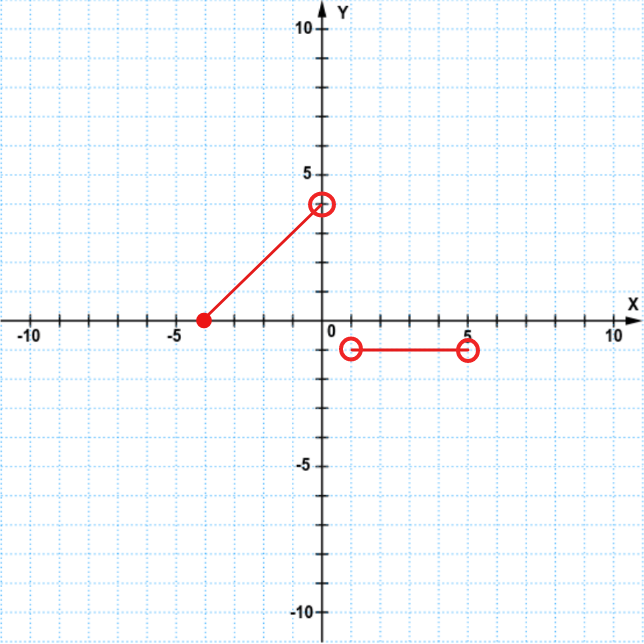
\includegraphics[width=0.8\linewidth]{wykres}
	\end{minipage}

\item \begin{tabular}{p{13cm} r}
	Rozwiąż równanie &[5pkt]\\ 
\end{tabular}

$$x^3-4x^2=3x-12$$

\end{enumerate}











	
\end{document}